\documentclass[12pt,a4paper]{article}
\usepackage{fontspec}
\usepackage{xcolor,graphicx,wrapfig,booktabs,amsmath,amsthm,enumitem,geometry,hyperref}
\geometry{margin=2.4cm}
\setmainfont{DejaVu Serif}
\renewcommand{\contentsname}{Садржај}
\renewcommand{\figurename}{Слика}
\renewcommand{\tablename}{Табела}
\newtheorem{definicija}{Дефиниција}
\newtheorem{lema}{Лема}
\newtheorem{teorema}{Теорема}
\title{\textbf{Развој технологије у MotoGP-у}}
\author{Јована Васиљевић — ми24183}
\date{Увод у информатику\\2026.}
\begin{document}
\maketitle
\tableofcontents
\newpage
\section{Увод}
\begin{wrapfigure}{l}{0.42\textwidth}
\centering
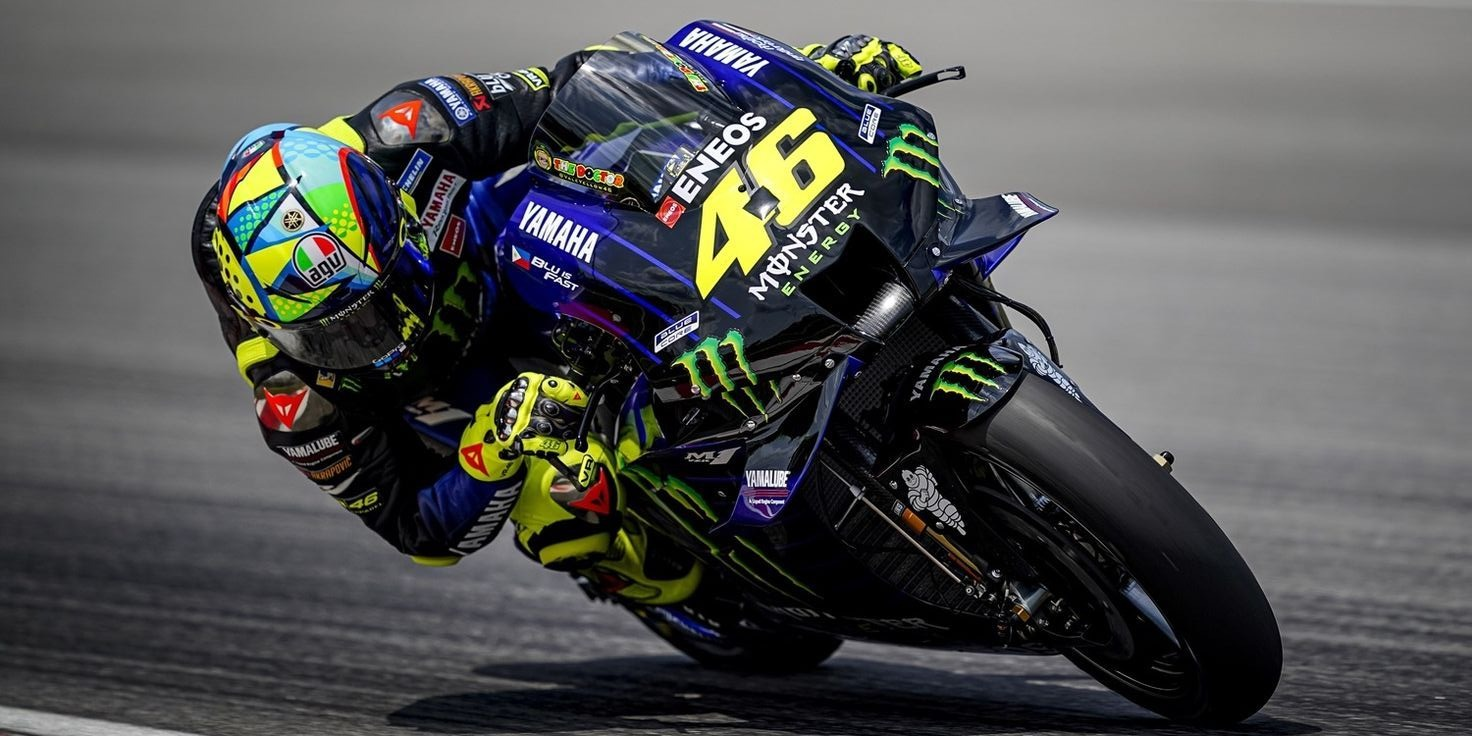
\includegraphics[width=0.40\textwidth]{slike/valentino-rossi.jpg}
\caption{Валентино Роси на мотоциклу са бројем 46}
\end{wrapfigure}
MotoGP представља врх мотоциклистичког спорта и важну лабораторију за развој нових решења. Валентино Роси, препознатљив по броју 46 и жутој боји, возио је у различитим епохама развоја тркачких прототипова.

\subsection{Основни појам}
\begin{definicija}
Тркачки прототип је возило развијено посебно за такмичење, без обавезе да буде засновано на серијском моделу.
\end{definicija}

\section{Кључне технологије}
При кретању, кинетичка енергија система може се представити формулом
\[
E_k=\frac{mv^2}{2},
\]
где су $m$ маса, а $v$ брзина. Формула показује зашто пораст брзине значајно повећава захтеве при кочењу.

\begin{lema}
Смањење масе уз задржавање крутости може побољшати промену правца и одзив мотоцикла.
\end{lema}
\begin{teorema}
Најбоље време круга не зависи од једног дела, већ од усклађеног рада возача, механике, аеродинамике, електронике и гума.
\end{teorema}

\subsection{Поређење система}
\begin{table}[h]
\centering
\begin{tabular}{lll}
\toprule
\textbf{Систем} & \textbf{Задатак} & \textbf{Резултат}\\
\midrule
Аеродинамика & Усмеравање ваздуха & Стабилност\\
Електроника & Обрада података & Контрола\\
Материјали & Мања маса и отпорност & Перформансе\\
\bottomrule
\end{tabular}
\caption{Улоге технолошких система}
\end{table}

Најважније области развоја су:
\begin{itemize}[label=--]
\item аеродинамички додаци и облик оплате;
\item сензори и анализа података;
\item карбонски композити и металне легуре.
\end{itemize}
Процес подешавања обично обухвата:
\begin{enumerate}
\item прикупљање података на стази;
\item анализу понашања мотоцикла;
\item промену подешавања и поновно тестирање.
\end{enumerate}

\section{Закључак}
\textcolor{red}{MotoGP показује колико су спорт и инжењерство повезани.} \textbf{Брзина је резултат читавог система}, а не само снаге мотора. \textit{Иновације, прецизност и безбедност} развијају се заједно, круг по круг.
\end{document}
